\documentclass[tikz,border=8pt]{standalone}
\usepackage{amsmath,amssymb}
\usetikzlibrary{arrows.meta,calc,decorations.pathreplacing,patterns,shapes.geometric,positioning,shadings}

% Rainbow palette for 8 channels (violet -> deep red)
\definecolor{chA}{HTML}{6A1B9A}
\definecolor{chB}{HTML}{1E88E5}
\definecolor{chC}{HTML}{00ACC1}
\definecolor{chD}{HTML}{43A047}
\definecolor{chE}{HTML}{FDD835}
\definecolor{chF}{HTML}{FB8C00}
\definecolor{chG}{HTML}{E53935}
\definecolor{chH}{HTML}{8E0B0B}

\definecolor{boxgray}{HTML}{EEEEEE}
\definecolor{muxfill}{HTML}{F5F5F5}

\begin{document}
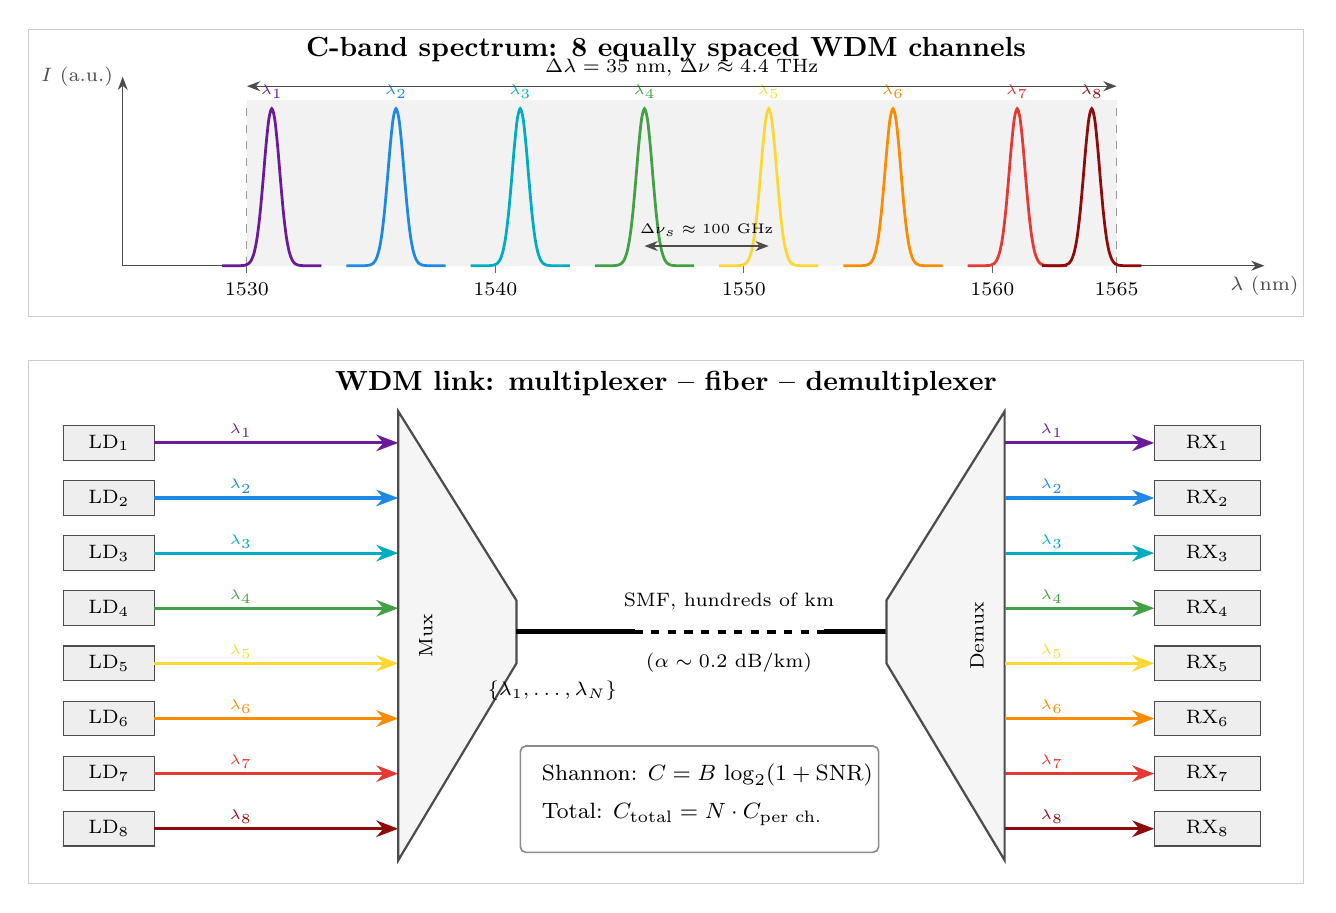
\begin{tikzpicture}[>=Stealth,font=\small]

% =====================================================
% Global layout
%   TOP:    spectrum panel  (y in [7.2, 10.8])
%   BOTTOM: WDM system schematic (y in [0, 6.6])
%   Formula box overlays lower-right corner
% =====================================================

% ======================================================
% PANEL A : Spectrum of C-band with 8 Gaussian peaks
% ======================================================
\begin{scope}[shift={(0,7.2)}]
  % Frame
  \draw[gray!40] (-0.1,-0.05) rectangle (16.1,3.6);
  \node[font=\bfseries] at (8.0,3.35) {C-band spectrum: 8 equally spaced WDM channels};

  % Plot area
  \def\sxL{1.1}
  \def\sxR{15.3}
  \def\syB{0.6}
  \def\syT{2.7}

  % Axes
  \draw[->,black!70] (\sxL,\syB) -- (15.6,\syB) node[anchor=north,font=\scriptsize] {$\lambda$ (nm)};
  \draw[->,black!70] (\sxL,\syB) -- (\sxL,3.0) node[anchor=east,font=\scriptsize] {$I$ (a.u.)};

  % x maps wavelength 1525..1570 nm linearly to [sxL,sxR]
  \foreach \lam in {1530,1540,1550,1560,1565}{
    \pgfmathsetmacro{\xx}{\sxL + (\lam-1525)/45 * (\sxR-\sxL)}
    \draw[black!60] (\xx,\syB) -- (\xx,\syB-0.09);
    \node[font=\scriptsize,anchor=north] at (\xx,\syB-0.09) {\lam};
  }

  % C-band shaded region
  \pgfmathsetmacro{\xcL}{\sxL + (1530-1525)/45 * (\sxR-\sxL)}
  \pgfmathsetmacro{\xcR}{\sxL + (1565-1525)/45 * (\sxR-\sxL)}
  \fill[black!5] (\xcL,\syB) rectangle (\xcR,\syT);
  \draw[black!40,dashed] (\xcL,\syB) -- (\xcL,\syT);
  \draw[black!40,dashed] (\xcR,\syB) -- (\xcR,\syT);

  % 8 Gaussian peaks at lambda centers
  \foreach \mu/\col/\idx in {%
      1531/chA/1,
      1536/chB/2,
      1541/chC/3,
      1546/chD/4,
      1551/chE/5,
      1556/chF/6,
      1561/chG/7,
      1564/chH/8}
  {
    \pgfmathsetmacro{\muLo}{\mu-2.0}
    \pgfmathsetmacro{\muHi}{\mu+2.0}
    \draw[\col,line width=1.0pt,smooth,domain=\muLo:\muHi,samples=35,variable=\l]
      plot ({\sxL + (\l-1525)/45 * (\sxR-\sxL)},
            {\syB + 1.9*exp(-pow((\l-\mu)/0.45,2)) * (\syT-\syB)/2.0});
    \pgfmathsetmacro{\xpk}{\sxL + (\mu-1525)/45 * (\sxR-\sxL)}
    \pgfmathsetmacro{\ypk}{\syB+0.95*(\syT-\syB)}
    \node[font=\tiny,text=\col,anchor=south] at (\xpk,\ypk) {$\lambda_{\idx}$};
  }

  % Annotation: C-band width
  \draw[<->,black!70] (\xcL,\syT+0.18) -- (\xcR,\syT+0.18);
  \node[font=\scriptsize,anchor=south] at ({(\xcL+\xcR)/2},\syT+0.18)
    {$\Delta\lambda = 35$ nm, $\Delta\nu \approx 4.4$ THz};

  % Channel spacing between channel 4 and 5
  \pgfmathsetmacro{\xpD}{\sxL + (1546-1525)/45 * (\sxR-\sxL)}
  \pgfmathsetmacro{\xpE}{\sxL + (1551-1525)/45 * (\sxR-\sxL)}
  \draw[<->,black!70] (\xpD,\syB+0.25) -- (\xpE,\syB+0.25);
  \node[font=\tiny,anchor=south] at ({(\xpD+\xpE)/2},\syB+0.25)
    {$\Delta\nu_s \approx 100$ GHz};

\end{scope}

% ======================================================
% PANEL B : WDM system schematic
% ======================================================
\begin{scope}[shift={(0,0)}]
  % Frame
  \draw[gray!40] (-0.1,-0.05) rectangle (16.1,6.6);
  \node[font=\bfseries] at (8.0,6.3) {WDM link: multiplexer -- fiber -- demultiplexer};

  % ---- Left side: 8 laser diodes ----
  \def\ldX{0.35}
  \def\ldW{1.15}
  \foreach \i/\yc/\col in {%
      1/5.55/chA,
      2/4.85/chB,
      3/4.15/chC,
      4/3.45/chD,
      5/2.75/chE,
      6/2.05/chF,
      7/1.35/chG,
      8/0.65/chH}
  {
    \draw[black!70,fill=boxgray] (\ldX,\yc-0.22) rectangle (\ldX+\ldW,\yc+0.22);
    \node[font=\scriptsize] at (\ldX+\ldW/2,\yc) {LD$_{\i}$};
    \draw[\col,line width=1.1pt,->] (\ldX+\ldW,\yc) -- (4.6,\yc);
    \node[font=\tiny,text=\col] at (\ldX+\ldW+1.1,\yc+0.15) {$\lambda_{\i}$};
  }

  % ---- Mux trapezoid (wide on left, narrow on right) ----
  \def\muxXL{4.6}
  \def\muxXR{6.1}
  \def\muxYT{5.95}
  \def\muxYB{0.25}
  \def\muxYTR{3.55}
  \def\muxYBR{2.75}
  \fill[muxfill] (\muxXL,\muxYB) -- (\muxXL,\muxYT) -- (\muxXR,\muxYTR) -- (\muxXR,\muxYBR) -- cycle;
  \draw[black!70,line width=0.8pt]
    (\muxXL,\muxYB) -- (\muxXL,\muxYT) -- (\muxXR,\muxYTR) -- (\muxXR,\muxYBR) -- cycle;
  \node[font=\scriptsize,rotate=90] at (\muxXL+0.35,{(\muxYT+\muxYB)/2}) {Mux};

  % ---- Single fiber ----
  \def\fyc{3.15}
  \def\fxA{6.1}
  \def\fxWavyL{7.6}
  \def\fxWavyR{10.0}
  \def\fxB{10.8}
  \draw[black,line width=1.8pt] (\fxA,\fyc) -- (\fxWavyL,\fyc);
  \draw[black,line width=1.5pt,dashed]
    (\fxWavyL,\fyc) -- (\fxWavyR,\fyc);
  \draw[black,line width=1.8pt] (\fxWavyR,\fyc) -- (\fxB,\fyc);

  \node[font=\scriptsize,anchor=south] at ({(\fxWavyL+\fxWavyR)/2},\fyc+0.15)
    {SMF, hundreds of km};
  \node[font=\scriptsize,anchor=north] at ({(\fxWavyL+\fxWavyR)/2},\fyc-0.15)
    {($\alpha \sim 0.2$ dB/km)};

  % ---- Demux trapezoid ----
  \def\dxL{10.8}
  \def\dxR{12.3}
  \def\dyTL{3.55}
  \def\dyBL{2.75}
  \def\dyTR{5.95}
  \def\dyBR{0.25}
  \fill[muxfill] (\dxL,\dyTL) -- (\dxR,\dyTR) -- (\dxR,\dyBR) -- (\dxL,\dyBL) -- cycle;
  \draw[black!70,line width=0.8pt]
    (\dxL,\dyTL) -- (\dxR,\dyTR) -- (\dxR,\dyBR) -- (\dxL,\dyBL) -- cycle;
  \node[font=\scriptsize,rotate=90] at (\dxR-0.35,{(\dyTR+\dyBR)/2}) {Demux};

  % ---- Right side: 8 receivers ----
  \def\rxX{14.2}
  \def\rxW{1.35}
  \foreach \i/\yc/\col in {%
      1/5.55/chA,
      2/4.85/chB,
      3/4.15/chC,
      4/3.45/chD,
      5/2.75/chE,
      6/2.05/chF,
      7/1.35/chG,
      8/0.65/chH}
  {
    \draw[\col,line width=1.1pt,->] (\dxR,\yc) -- (\rxX,\yc);
    \draw[black!70,fill=boxgray] (\rxX,\yc-0.22) rectangle (\rxX+\rxW,\yc+0.22);
    \node[font=\scriptsize] at (\rxX+\rxW/2,\yc) {RX$_{\i}$};
    \node[font=\tiny,text=\col] at (\dxR+0.6,\yc+0.15) {$\lambda_{\i}$};
  }

  % Combined-beam label on fiber (placed below, to left of descriptive text)
  \node[font=\scriptsize,anchor=north east] at (\fxWavyL-0.1,\fyc-0.5)
    {$\{\lambda_1,\dots,\lambda_N\}$};

\end{scope}

% ======================================================
% FORMULA BOX (centered below the fiber, between Mux and Demux)
% ======================================================
\begin{scope}[shift={(6.15,0.35)}]
  \draw[black!45,line width=0.6pt,fill=white,rounded corners=2pt]
    (0,0) rectangle (4.55,1.35);
  \node[font=\footnotesize,anchor=north west] at (0.15,1.25)
    {Shannon:  $C = B\,\log_2(1+\mathrm{SNR})$};
  \node[font=\footnotesize,anchor=north west] at (0.15,0.75)
    {Total:   $C_{\text{total}} = N \cdot C_{\text{per ch.}}$};
\end{scope}

\end{tikzpicture}
\end{document}
